\setcounter{chapter}{8}
\setchapterabstract{This chapter outlines the application of Article 101 of the Treaty on the Functioning of the European Union (TFEU), which prohibits anti-competitive agreements, decisions, and practices. Article 101(1) lists behaviours that may restrict competition, such as price-fixing, market sharing, and limiting production, while Article 101(3) allows exemptions if agreements create pro-competitive benefits like efficiency gains or improved product quality. These exemptions require that the benefits be passed on to consumers, and that the restrictions are necessary. Restrictions by "object" need no proof of anti-competitive effects, while others require a detailed market impact analysis. The chapter also highlights the "\textit{de minimis}" threshold, block exemptions, and the balance between restrictions and potential benefits under Article 101(3).}
\chapter{Cartels, CoOp Agreements and Information Exchanges}
\vspace{-1.5cm}

{\chaptoc\noindent\begin{minipage}[inner sep=0,outer sep=0]{0.9\linewidth}\section*{Cartels and the theory of collusion}\end{minipage}}

        \subsubsection{Why}

            Where a rather small number of rival firms\(^1\), selling a similar product, conclude that it is in their joint interests to collude rather than compete, they may establish a cartel arrangement in which they agree to set an industry price and output which enables them to achieve a monopolistic equilibrium. Absent antitrust laws, cartels would be always optimal from an industry point of view. 
            
           A. SMITH, \textit{The Wealth of Nations} (1776):

            \begin{quote}
                 “People of the same trade seldom meet together, even for merriment and diversions, but the conversation end in a conspiracy against the public, or in some contrivance to raise prices” .
            \end{quote}

        \subsubsection{How}

            This is likely to involve the setting of agreed output quotas for each member to maintain the agreed (monopolistic) price. The allocation of market quotas between members could be decided by different criteria, such as geography, productive capacity or pre-cartel market share (usually it is difficult to find an equilibrium between participants; furthermore, they may have to include inefficient firms and thus even the collusive equilibrium may be suboptimal; this is a further cost imposed to society).

        \hrulefill
        \newline
        \(^1\) \Note{sometimes not so small; 345 firms fined in the Dutch Construction Cartel by the NMA}

        \subsubsection{However}

            Cartels tend to be rather fragile and may not last for very long\sn{\Remark{
            Threats to cartels: 
            \begin{enumerate}[label=\alph*.]
                \item Asymmetry/different costs between members;
                \item Cheating;
                \item Technological progress;
                \item Possible entry;
                \item Demand fluctuations and/or dropping demand;
            \end{enumerate}
            }}. This is because individual members may have an incentive to deviate from the agreement by secretly undercutting the cartel price. The necessity to limit output to keep price high will tend to leave individual firms with spare productive capacity and provide the temptation to increase profits by expanding output + Out of area competitors may be attracted by profits realized in the market because of the functioning of the cartel. Such an expansion would not only generate profit on the additional sales, but would also increase the profits on existing sales, as average fixed costs would fall as output expanded.

            Thus, if you want to form an effective cartel, you need:

            \begin{itemize}
                \item to create and maintain trust between all the partners;
                \item to put in place monitoring mechanisms\sn{\Note{to detect possible cheating}}
                \item retaliation schemes if a firm deviates from agreed upon behaviour, the other cartelists should punish the deviation; thus, you must identify a credible threat/punishment mechanism against cheating.
            \end{itemize}

            The phrase “Our competitors are our friends, and our customers are our enemies”, was first used by ADM director Mark Whitacre in a Fortune magazine interview in 1996. Precisely the same aphorism was repeated by ADM President James Randall to Ajinomoto managers who were touring ADM’s lysine plant in Decatur, Illinois on April 30, 1993.

\section{Cartels}

    Here are a few quotes about cartels:
    \begin{itemize}
        \item M. Monti (2001), then Commissioner for Competition:
            \begin{quote}
                “Cartels are cancers on the open market economy”
            \end{quote}
        \item J. Klein (2002), A.A.G. Antitrust Division U.S. Department of Justice
            \begin{quote}
                “The reality is that price fixing, like bid-rigging and market allocation schemes, are anything but victimless crimes. The perpetrators of these conspiracies are, quite literally, stealing money out of the pockets of American businesses and consumers. ” Thus, the FIGHT against cartels (and bid rigging) is considered as the most important task of any antitrust authority”.
            \end{quote}
        \item R. Posner (N/A), U.S. Judge
            \begin{quote}
                "[Criminal sanctions against cartels] [...] are not really prices designed to ration the activity; the purpose so far as possible is to extirpate it"
            \end{quote}
    \end{itemize}

\newpage

    
    \begin{enumerate}
        \item \textbf{Price fixing}: price increases, target prices, rebates, costs, surcharges, price announcements. Price fixing is prohibited downstream but also upstream (buyers’ cartels: buyers agree on the “sell-in” price).
        
        \item \textbf{Market sharing}: Geographical market sharing; market sharing according to classes of customers; no active-aggressive competition agreements (“don’t touch my clients” rule). Geographical market sharing is considered a particularly serious infringement also because it may run contrary to the main EU Treaty goal (common market, and now internal market).
    
        \item \textbf{Quotas and other restrictions on production}: Client allocation (agreements are usually reinforced with monitoring and compensating payments in case of overriding the assigned quota); cross supplying on a continuous basis.
        
        \item \textbf{Collusive tendering/bid rigging}: A number of possible alternative schemes (rotate orders; tender sharing; preselection of the winning firm; respect for existing traditional customer relationships).
    
        \Example{
        In \textit{Elevators and Escalator}, the EU Commission imposed fines of €1 billion for bid-rigging, price fixing, and market allocation on maintenance of lifts and escalators in Belgium, Germany, and the Netherlands. The undertakings concerned informed each other of calls for tenders and coordinated their bids according to pre-agreed cartel quotas.
        }
        
        In some instances, \textbf{covert pricing} was used: bids that gave the pretense of competition but were deliberately set at a higher price than what would result from competition.

        \Example{
        ATM Milan (AGCM, 2001). Perfect allocation by reducing the number of parties from 15 to the number of tenders (12) via temporary partnerships and ventures; and then each party winning exactly one tender a year.
        }
    
        \item \textbf{Terms and conditions}: Non-price competition is very important too (part of the overall value of the good/service): after-sales services, financial conditions (see Italian alleged cartel on loans to buy cars); mandatory standard conditions of sales, etc. Any agreement on terms and conditions may thus restrict competition “appreciably” even if it does not directly refer to prices.
    
        \item \textbf{Advertising restrictions}: Advertising is a fundamental tool to get the attention of clients and thus try to increase sales and market shares (info about services, quality, and prices). A ban on advertising (or comparative advertising) may help maintain a “quiet life” between market participants. Many cases around Europe deal with advertising bans promoted by associations of professionals.
    
        \item \textbf{Collective group boycotts}: Against potential competitors or non-members of the cartel to guarantee cartel stability. These can be used to impede entry (especially when interconnection is needed – like in the payment system, telecoms system, etc.); or to push maverick firms out of the market (e.g., private security companies in Italy).
    \end{enumerate}

    \subsection{Vestager on the German carmakers cartels (22-10-2021): greenwashing}

        Sometimes, what we want as consumers is not so much a cheaper product as a better one. We want to be sure that the products we’re buying won’t harm the environment. So, a cartel that holds back improvements in the quality of the products we buy can be just as harmful as one that fixes prices.

        \textbf{July 2021}: The EU Commission took a decision against BMW, Volkswagen, and Daimler that limited competition on how effectively they would clean the exhaust of their diesel cars.
        
        The cartel took place within what was otherwise perfectly legal, even beneficial, technical cooperation. The companies were developing a new cleaning technology that used an additive, AdBlue, to reduce pollution, and they needed to cooperate to tackle some practical challenges – e.g., to set up a network of AdBlue filling stations.
        
        But they crossed the line into illegal collusion when they agreed that they wouldn’t aim at cleaning beyond the minimum level required by the legal standard.
        
        They knew they could remove even more pollution than the law required, by injecting more AdBlue. So, they could have competed to attract environmentally-conscious consumers, by making even cleaner cars. But instead, they chose not to compete for the best possible cleaning performance.
        
        \textbf{Fine}: 875 million €.

        \subsubsection{Cartel Fines}

            In the last years, the EU Commission fined:
            \begin{itemize}
                \item Truck producers cartel: €2.93B;
                \item 6 car air conditioning and engine cooling suppliers: €155M (settlement);
                \item 3 companies: €68M for car battery recycling cartel;
                \item Crédit Agricole, HSBC, and JPMorgan Chase: €485M for euro interest rate derivatives cartel;
                \item Car parts producers: €137.8M (settlement);
                \item Parking heaters producer: €68M (settlement);
                \item Cargo train operators: €49M;
                \item Suppliers of optical disc drives: €116M for cartel;
                \item Producers and distributors: €115.9M for operating retail food packaging cartels;
                \item Three producers of canned mushrooms: €32M (settlement);
                \item Car and truck bearings: €953M (settlement);
                \item Steel abrasives: €30.7M (settlement);
                \item Smart card chips producers: €138M;
                \item RBS-JPMorgan derivatives based on Swiss franc LIBOR (settlement);
                \item €61.6M fine on JPMorgan - broker ICAP: €14.9M for participation in several cartels in Yen interest rate derivatives;
                \item €32M bid-ask spreads charged on Swiss Franc interest rate derivatives;
                \item Five envelope producers: €19.4M (settlement);
                \item €31.6M Canned Vegetables;
                \item €16M Steel bars;
                \item €1.07B foreign exchange spot trading;
                \item €368M car safety equipment (seat belts, airbags, steering wheels);
                \item €546M for maritime car carriers;
                \item Car parts supplies (braking systems, spark plugs, etc): €260M for ethylene producers (settlement).
            \end{itemize}

            In the same period, the network of national competition authorities fine hundreds of cartels and naked restrictions.

\section{Horizontal Cooperation Agreements}

    \textbf{Legal Sources}: Block exemptions + Guidelines on the Applicability of Article 101 to Horizontal cooperation agreements (2023) + Guidelines on Article 101(3) (2004).
    
    Since 2004, almost no case law under Article 101(3), and the Commission has never applied Article 10 of Regulation 1/2003 (decisions stating that an arrangement does not infringe competition law).
    
    Thus, how can we assess the validity of a Horizontal Cooperation Agreement (HCA)?
    \begin{enumerate}[label=\alph*)]
        \item The agreement is not a naked restriction and is covered by the De Minimis Notice;
        \item The agreement is covered by a block exemption regulation (for example, the R\&D block exemption regulation); or
        \item By self-assessment of the agreement (Article 101(1) or 101(3)). The 2023 Guidelines on Horizontal Cooperation Agreements (HCO) are the main source of information and contain several very useful examples and scenarios.
    \end{enumerate}
    
    \Remark{
    \textbf{No presumption of harm to consumers}: HCAs can be a means to share risk, save costs, increase investments, pool know-how, enhance product quality and variety, and launch innovation faster.
    }

    \begin{itemize}
        \item Cooperation may assume many different forms: a mere contract, a structural contract (i.e: a contract that also provide for with some pooling of resources, and or cross-shareholding), the forming of a specific, mono-function joint venture.
        \item \textbf{Remember:} cooperation may lead to such levels of integration that it constitute a concentration: we discuss it in the last classes)
    \end{itemize}

    \subsection{Basic Principles}

        \begin{enumerate}
            \item R\&D Agreements;
            \item Production-Specialisation Agreements;
            \item Standardisation Agreements\sn{\Note{Sustainability agreements (that may take any of the previous forms, but mainly standardisation agreements)}};
            \item Purchasing Agreements;
            \item Commercialisation Agreements;
            \item Information Exchanges;
        \end{enumerate}

    \Remark{The closer an agreement is to the marketing phase, the higher the risk of a restriction of competition}

    A new notes on further HCA Guidelines (HCAG)
    \begin{enumerate}
        \item \textbf{HCAG are not quantitative}: No absolute negative presumptions, no prohibition thresholds. Reference to Market Shares are to be interpreted only as a first “indication” . Thus, more flexibility, even if at the cost of less legal certainty.
        \item HCAG contain formal distinctions between different types of agreement (R\&D; Specialisation; purchase; standardisation, etc.). However, Real life agreements can combine R\&D with Production, Purchasing with Information Exchange, etc. For these “Complex” agreements reference must be made to the rules laid down for the kind of agreement which represents the core of the cooperation (centre of gravity of integrated co-operation).
        \item Many types of cooperation between firms is not covered by HCAG However, HCAG are helpful because they state the general framework in which those agreements should be evaluated.
    \end{enumerate}

        \subsubsection{\textit{Bread and butter} antitrust analysis}

            In fact, we use the same two-stage analysis, i.e.:
            \begin{enumerate}[label=\alph*)]
                \item Has the agreement as its object or effect a restriction of competition?
                \item If there is a significant restriction of competition, can the parties prove that pro-competitive effects outweigh the restrictive ones?
            \end{enumerate}
            
            Cooperation agreements as such are not by object restrictions. However, a distinction must be drawn between:
            \begin{itemize}
                \item Agreements whose true aim is “cooperation” between otherwise independent competitors (which may restrict competition by effect, and in that event are usually eligible for exemption if market power is not excessive);
                \item Agreements used to disguise a cartel, or a naked restraint aimed at:
                \begin{itemize}
                    \item raising prices/limiting production;
                    \item facilitating collusion – e.g., via disclosure of strategic information;
                    \item artificially foreclosing third parties from the relevant market.
                \end{itemize}
                Those agreements are restrictive by object and usually don’t satisfy the 4 conditions laid down by Article 101(3).
            \end{itemize}

    \subsection{Always look at what’s sweeping under the carpet}

        In November 2019, the Commission opened an investigation to assess whether Casino and Intermarché have coordinated their conduct in breach of EU competition rules.

        Commissioner Vestager said:
        \begin{quote}
        “Buying alliances between retailers have become a key component of grocery supply chains. They can bring lower prices to consumers for food and personal care brands that they purchase daily. Such benefits can however disappear quickly if retailers use these alliances to collude on their sales activities. The Commission will therefore investigate if Casino and Intermarché have coordinated their activities in an anticompetitive way.”
        \end{quote}
        
        The Commission found that Casino and Intermarché went beyond the purpose of their alliance and engaged in anticompetitive conduct, by coordinating their activities on the development of their shop networks and their pricing policy towards consumers.
        
        The joint purchasing alliance was finally abandoned.
        

\section{Production/Specialisation agreements}

    Two or more parties active on the same product market agree to cease the production of certain products (usually inputs or intermediate products) and to purchase them from the other party (or from a common JV), who agrees to produce and supply those products.
    
    The main competition concerns are:
    \begin{enumerate}[label=\alph*)]
        \item A direct restriction of competition between the parties, even if they produce and market the final products independently;
        \item Coordination of the parties’ competitive behaviour downstream, in particular when the production agreement leads to a high commonality of their variable costs (i.e., the production cost of the input represents a very high percentage of total costs), and to sharing information on quantities;
        \item Foreclosure of competitors\sn{\Note{\textbf{Article 4 of the Block Exemption Regulation}: exemption is not available if the agreement contains some severe restrictions of competition like:
        \begin{itemize}
            \item Price fixing,
            \item Limitation of output or sales,
            \item Allocation of markets or customers (in these cases we have a by-object restriction).
        \end{itemize}
        To determine whether there is a restriction by effect, a counterfactual must be identified.}}.
    \end{enumerate}

        \begin{itemize}
            \item If the agreement enables the parties to enter a market that they would have otherwise been unable to enter, the agreement does not have any restrictive effect.
            \item No problem if the parties lack market power. No safe harbors, but for “specialization agreements” (similar to production agreements) there is a 20\% threshold in the Block Exemption.
            \item Even if the parties have a combined market share of over 20\%, there is no problem where the agreement leads to strong efficiencies (e.g., reducing variable costs, increasing capacity, improving the quality of a product) and the relevant market is dynamic, i.e., where there is a very high entry rate or market positions change frequently.
            \item Contract flexibilities are very important (examples to be discussed: (a) more than 2 participants; (b) no restrictions on sales by the JV to third parties; (c) Chinese walls on information sharing).
        \end{itemize}

    \subsection{Mock 1: new car batteries production plant}

        \textbf{Situation:} Arta and Bosk, suppliers of car batteries, decide to close down their old production plants and build a larger and more efficient plant run by a joint venture (JV), which will have a higher capacity than the total capacity of the old plants of A and B.

        No other capacity investment is planned by competitors C, D, E, which are using their facilities at full capacity.
        
        A and B have market shares of 20\% and 25\% respectively. Their products are the closest substitutes in a specific segment of the market (batteries for diesel cars), which is concentrated. The market is transparent and rather stagnant, there is no entry, and the market shares have been stable over time.
        
        \begin{itemize}
            \item \textbf{Production costs} constitute a major part of A and B's variable costs. 
            \item \textbf{Commercialisation is a minor} economic activity in terms of \textbf{costs} and strategic importance compared to production: marketing costs are low as car batteries are a homogeneous and established product, and demand is relatively inelastic, and transport is not a key driver of competition.
        \end{itemize}

        \subsubsection{Analysis}

            If A \& B share most of their variable costs, this production agreement could lead to a direct limitation of competition between them. In fact:

            \begin{enumerate}[label=\alph*)]
                \item Given the combined market power of A \& B, the agreement may lead the parties to limit the output of the JV compared to what they would have brought to the market if each of them had decided its output on its own. Considering that they were close competitors and competitors’ capacity constraints, the output reduction could lead to higher prices.
                \item Given that A \& B share a significant part of their variable costs, this agreement can lead to a collusive outcome between A and B. The likelihood of this depends not only on the issue of commonality of costs (high in this case), input information sharing, but also on the characteristics of the relevant market such as transparency, stability, and the level of concentration.
            \end{enumerate}
            
            In either of the two situations, it is likely that the production JV would give rise to restrictive effects on competition within the meaning of Article 101(1).
            
            However, the replacement of two old production plants with a larger and more efficient one may lead the JV to increase output at lower prices to the benefit of consumers. The production agreement could only meet the criteria of Article 101(3) if the parties provide strong evidence that the efficiency gains would be passed on to consumers to such an extent that they would outweigh the restrictive effects on competition.

    \subsection{Mock 2: risk of foreclosure}

        A and B are important producers of dark lenses and sunglasses. They want to set up a joint venture (JV) to produce dark lenses, which will cover their entire production of dark lenses (thus, they will cease to compete in the upstream market).

        \begin{itemize}
            \item The production costs of dark lenses account for 70\% of the variable costs of the final product (sunglasses), with respect to which A and B compete downstream.
            \item A and B each have a share of 20\% in the market for sunglasses. In the past, there has been limited entry into the market. Market shares have been stable over time.
            \item In addition to covering their own demand for dark lenses, both A and B also sell dark lenses to other producers of sunglasses. "A" has a market share of 45\% and "B" has a market share of 35\% in the market for dark lenses (total sales, which include self-consumption).
            \item There are high barriers to entry in the market for dark lenses and existing producers are operating near full capacity.
            \item In the market for sunglasses, there are two other significant suppliers, each with a 15\% market share, and several smaller competitors.
            \item The agreement between A and B generates economies of scale in the upstream market.
        \end{itemize}

        \begin{center}
        \begin{tabular}{l|l|l|}
            Dark lenses & 45\% & 35\% \\
            \hline
            Sunglasses & 20\% & 20\% \\
            \hline
        \end{tabular}
        \end{center}

        \subsubsection{Analysis}

            By virtue of the production JV, A and B would be able to largely control supplies of an essential input (dark lenses) to their competitors in the market for sunglasses (together they will cover 80\% of the total supply- capacity of dark lenses). 
            
            This would give A and B the ability to raise their rivals’ costs by artificially increasing the price of dark lenses, or by reducing the output. 
            
            This could foreclose competitors of A and B in the market for sunglasses. Because of the likely anti-competitive foreclosure downstream, this agreement gives rise to restrictive effects on competition within the meaning of Art. 101(1). 
            
            The (possible) economies of scale generated by the production JV are unlikely to outweigh the (very likely) restrictive effects on competition; therefore, this agreement would most likely not meet the criteria of Art. 101(3).

\newpage
\section{Joint Purchasing Agreement}

    \Definition{
    A joint purchasing agreement refers to an arrangement where two or more companies or entities come together to purchase goods or services collectively, typically to leverage better terms from suppliers, such as lower prices or improved conditions due to the larger volume of purchase.
    While joint purchasing can be efficient and beneficial to consumers through lower costs, it may raise competition law concerns when it results in anti-competitive behaviour.
    \begin{enumerate}
        \item \textbf{Market power}: If the companies involved in the joint purchase have a large share of the market, they may have the ability to impose unfair conditions on suppliers, leading to distortions in the market.
        \item \textbf{Collusion risk}: There is a potential risk of collusion if joint purchasing arrangements extend beyond procurement into other areas, such as setting prices or output, which could lead to anti-competitive agreements that restrict competition.
    \end{enumerate}
    }{
    Joint Purchase Agreement
    }

        Two or more undertakings agree to jointly buy one or several items from the same seller. Joint purchasing agreements (JPA) aim at creating more buyer power to obtain lower purchasing prices, but also efficiencies in transaction, transport, logistics, and storage costs (e.g., supermarket chains form central purchasing bodies to negotiate lower prices with big suppliers such as Coca-Cola, Colgate, Procter \& Gamble, etc.).

        Thus, buyers’ associations will pay less for those products and may become more competitive downstream. At the same time:
        \begin{enumerate}[label=\alph*)]
            \item They will standardize the level of costs (same variable costs), and
            \item They may become aware of the quantities purchased by competitors (information sharing through the central body).
        \end{enumerate}
        
        The main antitrust concerns in the downstream market are:
        \begin{itemize}
            \item If the parties enjoy market power, they have no incentive to pass on to consumers any lower price they extract from suppliers (and information sharing on quantities can increase the danger of a quiet-life attitude).
            \item Furthermore, the agreement may lead to a possible reduction in variety (since they buy from the same suppliers).
        \end{itemize}

        \subsubsection{In the upstream market}

            \begin{enumerate}[label=\alph*)]
                \item If the parties have significant market power, by pushing to reduce the sell-in price, they can force their suppliers to reduce the range or quality of the goods they produce.
                \item They can raise their rival costs (producers, obliged to undercut prices due to buyer power, may increase the selling price to parties outside the purchasing agreement).
                \item They may cause foreclosure of competing purchasers by limiting their access to efficient suppliers.
            \end{enumerate}
            
            It’s unlikely that Article 101(1) would be infringed where market shares in both the purchasing and selling markets are below 15\%, and, in any case, the conditions of Article 101(3) would likely be fulfilled.
            
            Furthermore, some of the described competitive risks may be reduced by contractual provisions:
            \begin{itemize}
                \item Chinese walls on data;
                \item Allowing a second contractual phase between the parties and the producers;
                \item Allowing for flexibility on products and quantities;
                \item Limiting the cooperation to certain products/categories (preserving competition on the range of products).
            \end{itemize}

    \subsection{Mock 1: small purchasers}

        \textbf{Situation}: 150 small retailers reach an agreement to form a joint purchasing body.

        They are obliged to purchase a minimum volume through the organisation, which accounts for roughly 50\% of each retailer’s total costs. The retailers can purchase more than the minimum volume through the organisation.
        
        The retailers have a combined market share of 23\% on both the purchasing and selling markets. Company A and B are their two largest competitors. "A" has a 25\% share on both the purchasing and selling markets; "B" has a 35\% share on those markets.
        
        There are no barriers that would prevent the remaining small competitors from also forming a purchasing group.
        
        The 150 retailers achieve substantial cost savings by purchasing jointly through the purchasing organisation.

        \subsubsection{Analysis}

            The retailers have only a moderate market position on the purchasing and the selling markets.  
            
            Furthermore, the cooperation brings about some economies of scale.  
            Even though the retailers achieve a high degree of commonality of costs, they are unlikely to have market power on the selling market due to the market presence of Companies A and B, which are both individually larger than the joint purchasing organisation.
            
            Consequently, the retailers are unlikely to coordinate their behaviour and reach a collusive outcome.  
            The formation of the joint purchasing organisation is therefore unlikely to give rise to restrictive effects on competition within the meaning of Article 101. On the contrary, it may increase competition in the market.

        \subsection{Mock 2: big supermarket chains}

            \textbf{Situation}:  
            Carrefour and Auchan, two giant French supermarket chains, sign an agreement to jointly purchase products which account for roughly 80\% of their variable costs. The agreement covers all the mass-market products.
            
            On the relevant purchasing markets for the different categories of products, the parties have combined market shares between 35-40\%. On the relevant selling markets (supermarket channel), they have a combined market share of 60\%.
            
            In France, there are 3 other significant retailers, each with a 10\% market share, and some smaller ones. Market entry is not likely.

            \subsubsection{Analysis}

                The Joint Purchasing Agreement (JPA) increases the parties’ ability to coordinate their behaviour on the selling market, thereby leading to a collusive outcome. The parties have significant market power on the selling market (60\%) and the JPA gives rise to a significant commonality of costs (and information sharing).

                Moreover, market entry is unlikely in the short run. The incentive for the parties to coordinate their behaviour would be reinforced if their cost structures were already similar prior to concluding the JPA.
                
                Hence, the JPA is likely to give rise to restrictive effects on competition within the meaning of Article 101(1).
                
                More negative effects could be envisaged on the purchasing markets (this also depends upon the relative strength of producers\ldots).
                
                Even though the JPA is very likely to give rise to some efficiency gains in the form of cost savings, due to the parties’ significant market power on the selling market these are unlikely to be passed on to consumers to an extent that would outweigh the restrictive effects on competition.
                
                Therefore, the JPA is unlikely to fulfil the criteria laid down by Article 101(3).
                
\section{Information Exchanges}

    \textit{Information Exchange} may also lead to efficiency gains. Information about competitors’ costs can enable companies to become more efficient if they benchmark their performance against the best practices in the industry and design internal incentive schemes accordingly. Exchange of consumer data between companies in markets with asymmetric information about consumers can also give rise to efficiencies. E.g.: keeping track of the past behaviour of customers in terms of accidents or credit default provides an incentive for consumers to limit their risk exposure. 
    
    It also makes it possible to detect which consumers carry a lower risk and should benefit from lower prices. Consumers need information to make a weighted decision. Thus, IE may allow consumers to carry out their fundamental selective function in a more thoughtful way (think at website platforms like skyscanner, booking.com, etc.).

    The first step of the analysis is to put the IE in context; There are three different situations, in (A) and (B) IE is ancillary to other categories of agreements.

        \begin{enumerate}
            \item[a)] \textbf{IE in support of a horizontal cooperation agreement} (i.e., a specialization agreement, an R\&D agreement) or a vertical agreement. If the IE is strictly necessary to run the agreement (exchange of information about the complementary technologies used to boost R\&D for a new product), the IE is analysed together with the cooperation agreement. If the cooperation agreement is not caught by Article 101, also the IE is not caught.
            \item[b)] \textbf{IE in support of a cartel} – a mechanism for monitoring or enforcing compliance with an unlawful cartel agreement. The IE is considered as part of the overall anticompetitive behaviour (it may contribute to increase the seriousness of the restriction, reflecting the aim of cartel participants to effectively monitor and punish cheaters).
            \item[c)] \textbf{“Pure” agreements to exchange information}. Example:\sn{\Example{Consider the following example in a two competitors’ game environment: \begin{enumerate}[label=\alph*]
                \item Demand is known;
                \item Level of production/sales in order to reach; monopolistic equilibrium is known ($Q_m$); 
                \item Then, if your competitor tells you that it is going to produce $Q_1$, you also know that in order to reach a monopolistic equilibrium you should produce $Q_2 = Q_m – Q_1$ 
            \end{enumerate} 
            You may think at different examples, like a price increase announcement by the market leader in a leader/followers market environment.}} an association of undertaking collects data about its members’ sales, costs, prices, etc., elaborate it and give it back to its members. In this context IE can restrict competition either “by object” or “by effect”
                \begin{enumerate}
                    \item[i.] \textbf{By Object:} Information on future prices and/or quantities. In this case there is no need of further agreements between the parties on price or price increases. The mere fact of providing this kind of strategic information to other parties is likely to be sufficient for a finding of an agreement on prices (recall: internal use of information is presumed)\sn{\Example{Back in 2013, in “LIBOR” the EU Commission imposed fines totaling €1.49 billion on banks informing each other of their strategies and submissions for the calculation of the LIBOR rates. As we have seen, in July 2024 in “Portuguese banks” the CJEU confirmed that such exchanges are prohibited by object.}}.
                    
                    \item[ii.] \textbf{By Effect:} CJEU, C-238/05, Asned-Equifax: IE compatibility with antitrust law cannot be assessed in the abstract. It depends on \dots
                    \begin{itemize}
                        \item[(i)] the economic conditions on the relevant markets, and
                        \item[(ii)] the specific characteristics of the system concerned, such as:
                        \begin{itemize}
                            \item its purpose;
                            \item the conditions to access to it;
                            \item participation in it;
                            \item as well as the type of information exchanged -- be that public or confidential, aggregated or detailed, historical or current;
                            \item the periodicity of such information, and
                            \item its importance for the fixing of prices, volumes or conditions of service.
                        \end{itemize}
                    \end{itemize}
                \end{enumerate}
        \end{enumerate}

        \Remark{The question is, thus: when do IEs reduce or remove uncertainty between undertakings on their reciprocal strategies and decisions so that competition may be restricted by effect?}

    \subsection{Economic conditions}

        \textbf{Economic conditions of the relevant markets.} If markets are already transparent, concentrated, non-complex, symmetric, and stable, it is likely that IE on strategic data leads to a restriction (collusive coordination).  
        
        Tight oligopolies can facilitate a collusive outcome on the market as it is easier for fewer companies to reach a common understanding on the terms of coordination and to monitor deviations.   With more companies coordinating, the gains from deviating are greater because a larger market share can be gained through undercutting. Collusive coordination is thus less likely and less stable.  
        
        This does not mean that coordination through IE is a priori impossible in non-concentrated markets. If regulation plays a strong role on the market, IE on the few non-regulated strategic variables may lead to collusion also in a non-concentrated market.

    \subsection{Information Characteristics}

        \begin{enumerate}
            \item \textbf{Strategic information:\sn{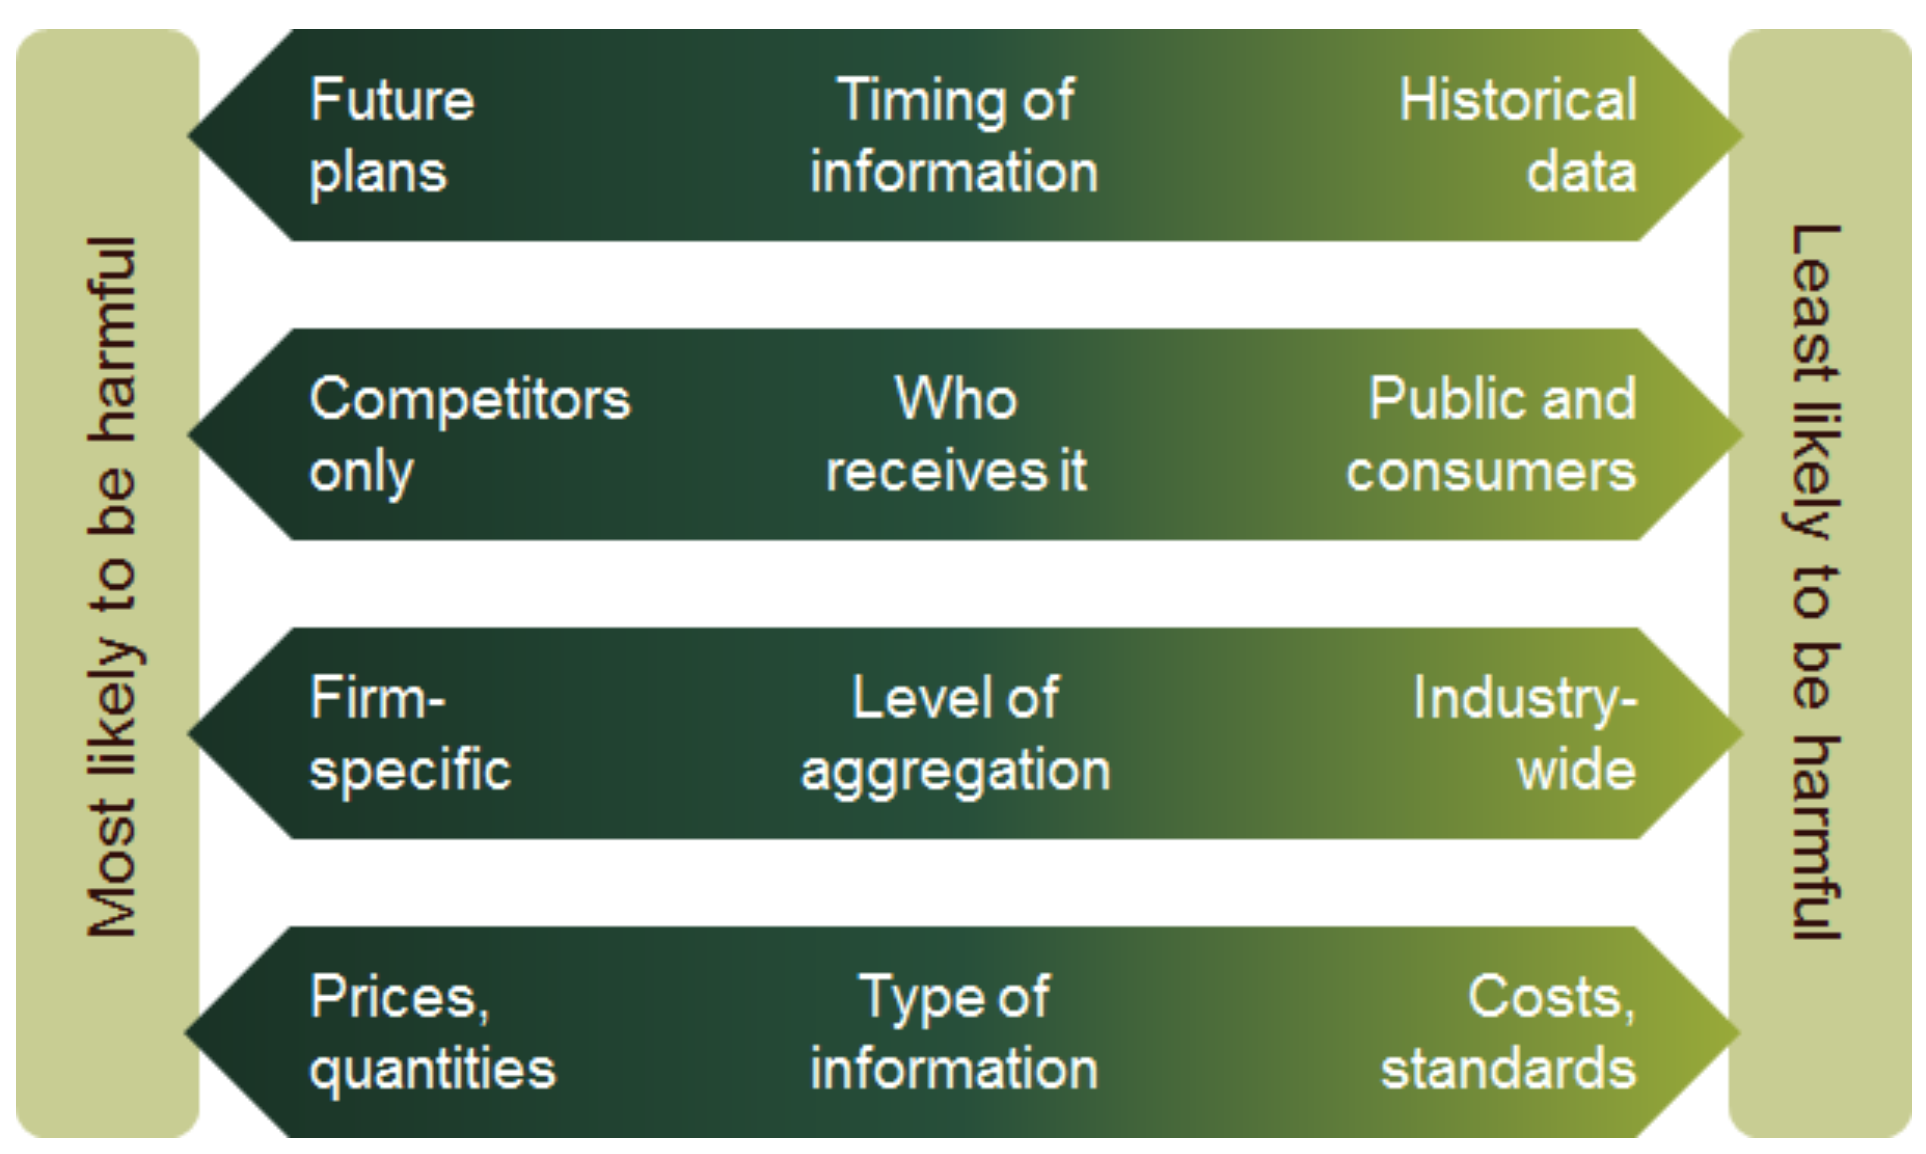
\includegraphics[width=1\linewidth]{strategic_information.png}}} The exchange of strategic data, i.e., data that reduces strategic uncertainty in the market, is more likely to be caught by Art. 101. Strategic information can be related to prices (discounts, rebates, increases), customer lists, production or distribution costs, quantities, turnovers, sales, capacities, qualities, marketing plans, risks, investments, technologies, and R\&D programs and their results.
                        
            \item \textbf{Market coverage:} For an IE to be likely to have restrictive effects on competition, the companies involved in the exchange must cover a sufficiently large part of the relevant market.
            
            \item \textbf{Aggregated/Individualized data:} Exchanges of genuinely aggregated data, where recognition of individualized company-level information is sufficiently difficult, are less likely to lead to restrictive effects on competition than exchanges of company-level data.  
            Conversely, exchanges of individualized data facilitate a common understanding on the market and punishment strategies by allowing colluding companies to single out a deviator or entrant.
            
            \item \textbf{Age of data:} The exchange of historic data is unlikely to lead to a collusive outcome as it is unlikely to be indicative of the competitors’ future conduct or to provide a common understanding on the market.
            
            \item \textbf{Frequency of the information exchange:} Frequent IEs that facilitate both a better common understanding of the market and monitoring of deviations increase the risks of a collusive outcome.
            
            \item \textbf{Public/non-public information:} Genuinely public information is generally equally accessible to all competitors and customers. For information to be genuinely public, obtaining it should not be more costly for customers and companies unaffiliated to the exchange system than for the companies exchanging the information. Public information means lower risk of determining a collusive outcome on the market.
            
            \item \textbf{Public/non-public exchange of information:} An IE is genuinely public if it makes the exchanged data equally accessible (in terms of costs of access) to all competitors and customers. The fact that information is exchanged in public may decrease the likelihood of a collusive outcome on the market to the extent that non-coordinating companies and customers may be able to constrain potential restrictive effects on competition.
        \end{enumerate}

\newpage

    \begin{figure}[h!]
        \centering
        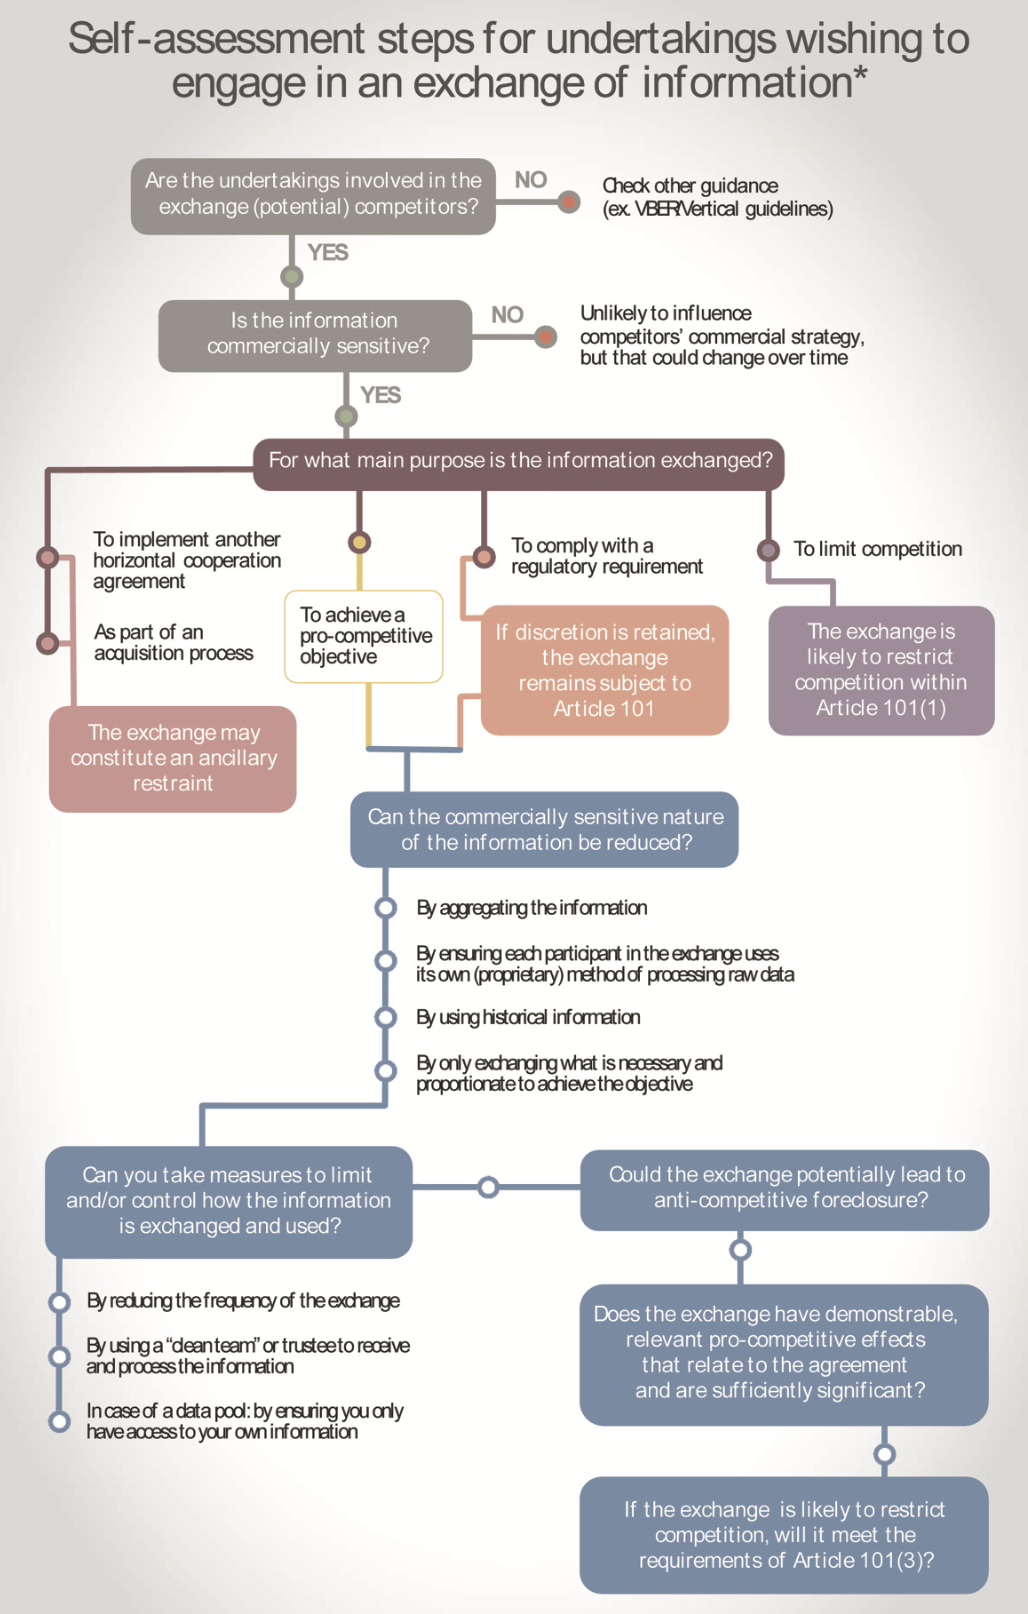
\includegraphics[width=1\linewidth]{Final_Info_Exchange.png}
    \end{figure}

\newpage

\section{Sustainability}

    Sustainable development is a core principle of the Treaty on EU and a priority objective for the Union’s policies. The Commission has committed to implement the UNs’ sustainable development goals. The European Green Deal sets out a growth strategy that aims to transform the Union into a fair and prosperous society, with a modern, resource-efficient and competitive economy\sn{\Note{no net emissions of greenhouse gases from 2050 onwards; economic growth is decoupled from resource excessive exploitation.}}.

    Sustainable development refers to the ability of society to consume the resources available today without compromising the ability of future generations to meet their own needs. It encompasses activities that support economic, environmental, and social development.
    \Remark{Sustainability is not only addressing climate change and pollution, but also limiting the use of natural resources, upholding human rights, ensuring a living income, fostering resilient infrastructure and innovation, reducing food waste, facilitating a shift to healthy and nutritious food, ensuring animal welfare, etc.}

    \subsection{Sustainability Agreements (SA)}

        Main Concern: Individual production and consumption decisions can have negative effects (`negative externalities'), e.g., on the environment, not sufficiently considered by the economic operators or consumers that cause them.

        This type of market failure can be mitigated by collective action, primarily through public policies or (sector-specific) regulation, and secondarily through cooperation agreements between undertakings that promote sustainable production or consumption.  
        Where such market failures are fully addressed by appropriate regulation, additional measures such as cooperation agreements may be unnecessary\sn{\Note{However, cooperation agreements may address residual market failures that are not or not fully addressed by public policies and regulation (i.e., they may anticipate, facilitate, speed up, or complete the reaching of those goals).}}.

    \subsection{Allowed SA}

        \begin{itemize}
            \item Agreements to ensure compliance with sufficiently precise requirements or prohibitions in legally binding international treaties, agreements, or conventions, whether or not they have been implemented in national law (for example, compliance with fundamental social rights or prohibitions on the use of child labor) and which are not fully implemented or enforced by a signatory State.
            
            \item Agreements that do not concern the economic activity of undertakings, but their internal corporate conduct. Competing undertakings may seek to increase the green reputation of their industry and for this purpose agree, e.g., on measures to eliminate single-use plastics from their business premises; etc.
            
            \item Agreements to set up a database containing general information about suppliers that have (un)sustainable value chains (for instance, suppliers that respect labor rights or pay living wages); use (un)sustainable production processes, etc., \textbf{IFF} they do not forbid or oblige the parties to purchase from such suppliers or to sell to such distributors.
            
            \item Agreements relating to the organization of industry-wide awareness campaigns, or campaigns raising customers' awareness of the environmental impact or other negative externalities of their consumption.
        \end{itemize}

    \subsection{Sanctioned SA}

        To contribute to sustainable development, competitors may agree:
        \begin{itemize}
            \item to phase out, withdraw, or replace non-sustainable products (e.g., coal) and processes (coal-fired steel production) with sustainable ones;
            \item to harmonize packaging materials to facilitate recycling or harmonize packaging sizes (and hence product content) to reduce waste;
            \item to purchase only production inputs that have been manufactured in a sustainable manner.
        \end{itemize}
        
        For these purposes, competitors may agree to adopt and comply with certain sustainability standards and production metrics.  
        SA usually provides rules, guidelines, or characteristics for products and processes in relation to such sustainability metrics.  
        The cost of complying with a sustainability standard can be high, particularly if this requires changes to existing production/distribution processes. Therefore, adhering to a sustainability standard may lead to an increase in production or distribution costs and consequently to an increase in the price of the products sold by the parties. It may also reduce variety.

\section{Soft Safe Harbour}

    SA may thus have some restrictive effect in terms of price increases, variety reduction, foreclosure of alternative standards, and exclusion of certain competitors.  
    However, the guidelines provide for a soft safe harbour if 6 cumulative conditions are met:
    \begin{enumerate}
        \item the procedure for developing the sustainability standard must be transparent; all interested competitors must be able to participate in the process leading to the selection of the standard;
        
        \item the sustainability standard must not impose on firms not wishing to participate in the standard any direct or indirect obligation to comply with the standard;
        
        \item to ensure compliance with the standard, binding requirements can be imposed on the participating firms, but they must remain free to apply higher sustainability standards;
        
        \item the parties must not exchange strategic information not necessary and proportionate for the development, implementation, adoption, or modification of the standard;
        
        \item effective and non-discriminatory access to the outcome of the standard-setting process must be ensured also to firms that didn’t participate in the development of the standard;
        
        \item the sustainability standard must satisfy at least one of the following two conditions:
        \begin{itemize}
            \item The standard must not lead to a significant increase in the price or a significant reduction in the quality of the products concerned;
            \item The combined market share of the participating undertakings must not exceed 20\% on any relevant market affected by the standard.
        \end{itemize}
    \end{enumerate}

    \subsection{Exemption 1: Efficiencies}

        If a SA does not satisfy the 6 conditions, then it must not be significantly restricting competition. If it falls under the Art. 101 prohibition, it can still benefit from an exemption.  
        First condition, the term efficiency is interpreted in wide terms:  
        \begin{quote}
            ``Examples of efficiencies that can be generated by SA include the use of less polluting production or distribution technologies, improved conditions of production and distribution, more resilient infrastructure, better quality products. SA can also reduce supply chain disruptions; shorten the time it takes to bring sustainable products to the market; enable consumers to make informed purchasing decisions by facilitating the comparison of products. These efficiency gains can contribute to a resilient internal market.''
        \end{quote}

        \Remark{Efficiencies need to be objective, concrete, and verifiable.}
        
        If the claimed efficiency is the reduction of water contamination, the parties must be able to explain how exactly the agreement contributes to the reduction of water contamination and provide an estimate of the magnitude of the claimed benefit.

    \subsection{Exemption 2: Pass-on to consumers}

        Three possible benefits. The first is the usual one:

        \subsubsection{1. Individual use benefits}

            Consumer benefits typically derive directly from consumption/use of the products covered by the agreement.
            \begin{itemize}
                \item vegetables that are cultivated using organic fertilizers may have better taste and/or be healthier for consumers than vegetables produced with non-organic fertilizers;
                \item replacing plastic in certain products with more durable materials may increase the longevity of the products in question.
            \end{itemize}
            
            In these circumstances, consumers enjoy greater quality simply by consuming the product in question. These are typical qualitative efficiencies that may be brought about by a restrictive agreement and may outweigh the harm caused by a price increase, or by a reduction in choice.  
            Thus, they may fulfil the second condition of Art. 101(3).

        \subsubsection{2. Altruistic benefits}

            Consumer benefits from SA may also consist of indirect benefits resulting from consumers' appreciation of the impact of their sustainable consumption on others.  
            Consumers may value their consumption of a sustainable product more than the consumption of a non-sustainable product because it has less negative impact on others.
            
            \Example{Consumers may opt for a particular washing liquid not because it cleans better but because it contaminates the water less.}
            
            \Example{Drivers may opt to use more expensive fuel not because it is of higher quality, but because it pollutes less.}
            
            The consumers' experience of the product is not directly improved. Nevertheless, they may be willing to pay a higher price for a sustainable product or to limit their choice of products (by not buying non-sustainable variants) to benefit society or future generations. Hence, indirect, non-use value benefits accrue to consumers within the relevant market via their individual valuation of the effect on others, including on non-users outside the relevant market.  
            Consumers willing to pay more for such products perceive them to be of a higher quality precisely because of the benefits accruing to others.

        \subsubsection{3. Collective Benefits}

            Not all negative externalities can be taken care of through voluntary, individual consumer actions.  
            As the sustainability impact from individual consumption accrues not necessarily to the consuming individual but to a larger group, a cooperation agreement may be needed to internalize negative externalities and bring about sustainability benefits for a wider section of society.

            \Example{Consumers don’t want to pay a higher price for a product manufactured with a green but costly technology. To ensure that the benefits derived from the use of that technology materialize, an agreement to phase out the polluting technology may be necessary.}
            
            These benefits are referred to as `collective benefits', as they occur irrespective of the consumers’ individual appreciation of the product and accrue to a wider section of society than just consumers in the relevant market.  
            However, according to Art. 101(3) the weighing of the pros and cons of the restrictive agreements is normally done within the relevant market to which the agreement relates.  
            The guidelines bypass the problem by saying that where consumers in the relevant market substantially overlap with (or form part of) the group of beneficiaries outside the relevant market, also the collective benefits to the consumers in the relevant market that occur outside that market can be considered if they are significant enough to compensate the consumers in the relevant market for the harm that they suffer.

            \Example{Drivers purchasing less polluting gasoline are also citizens who would benefit from cleaner air if less polluting gasoline were used.  
            If there is a substantial overlap of consumers (the drivers) and the wider beneficiaries (citizens), the sustainability benefits of cleaner air can be considered, if they compensate the consumers in the relevant market for the harm suffered.}
            
            The overlapping market criterion may make it harder to justify certain initiatives, i.e., agreements to stop using cotton from plantations outside the EU that employ toxic herbicides, where most of the negative externalities avoided (such as health risks to farmers) accrue to a different set of consumers or to society at large.
            
            The Guidelines suggest that such an agreement may not be justified under Article 101(3) TFEU, because the costs are borne by EU consumers, whereas the benefits of eliminating the toxic materials mainly accrue to communities outside the EU.
            
            This seems inconsistent with the worldwide scope of Article 3(5) TEU (the EU ``shall contribute to (…) the sustainable development of the Earth", and not just the EU).











